\documentclass{article}
\usepackage[utf8]{inputenc}
\usepackage{graphicx}
\usepackage{fancyhdr}
\usepackage{geometry}
\usepackage{amsmath}
\usepackage{amssymb}
\usepackage{url}
\usepackage{hyperref}

\geometry{left = 2.5cm, right=2.5cm, bottom=2.5cm, top=2.5cm}

\title{3806ICT - Exercises week 1 $\rightarrow$ 5}
\author{Nick van der Merwe - s5151332 - nick.vandermerwe@griffithuni.edu.au}

\pagestyle{fancy}
\renewcommand{\headrulewidth}{1pt}
\fancyhf{}
\rhead{3806ICT - Exercises w1-5}
\chead{Griffith University}
\lhead{Nick van der Merwe - s5151332}
\rfoot{Page \thepage}
\newcommand\tab[1][1cm]{\hspace*{#1}}

\begin{document}
\maketitle

%==============================================================================
\section*{Question 1}
% \textbf{\textit{
%     \tab Give  definitions  of  locomotion  and  manipulation.  What  are  their shared features and differences?  
% }} \\ \\
Locomotion is defined as a robot's ability to move itself by exerting force on 
the environment whereas manipulation is its ability to move objects by 
exerting force upon them. So their shared feature is that they exert force using
a mechanism, but their difference is what ends up moving. In locomotion, the
robot itself moves and in kinematics the other object moves.
%==============================================================================
\section*{Question 2}
% \textbf{\textit{
%     \tab What are advantages and disadvantages of legged robots?
% }} \\ \\
Easiest format to see this in would be lists:
\subsubsection*{Advantages}
\begin{itemize}
    \item They can go over more complicated obstacles without 
        getting stuck (slanted ground, steps, et cetera)
    \item Causes less damage to terrain than wheeled robots
\end{itemize}
\subsubsection*{Disadvantages}
\begin{itemize}
    \item Movement speed
    \item Complexity - actuators and structure are a lot more complicated
    \item Harder to control - must consider balance and stability
    \item Less energy efficient due to:
    \begin{itemize}
        \item Terrain
        \item Centre of gravity moves while walking
        \item Picking up the legs
    \end{itemize}
\end{itemize}
%==============================================================================
\section*{Question 3}
% \textbf{\textit{
%     \tab What is DOF? If a robot can only move forward and backward, 
%     how many DOFs does it have? In most cases, how many DOFs does a robot leg has?
% }} \\ \\
DOF stands for \textbf{d}egrees \textbf{o}f \textbf{f}reedom, and its defined by the
number of joins in each leg. To have a leg that only moves forwards and backwards,
it would have two joints: this is because its limited to doing a lift and swing motion.
To move backwards it just swings in the other direction than normal. Most robot legs
have three joints.
%==============================================================================
\newpage
\section*{Question 4}
% \textbf{\textit{
%     \tab What is a gait of a legged robot? Enumerate all lift and release 
%     events of a robot with 4 legs. Give two examples of gaits for such a robot.
% }} \\ \\
Our formula to find how many states there are is $2^k = 2^4 = 16$ states, so the
fact that Figure \ref{gait} has 16 states reinforces its validity.
\begin{figure}[ht]
    \centering
    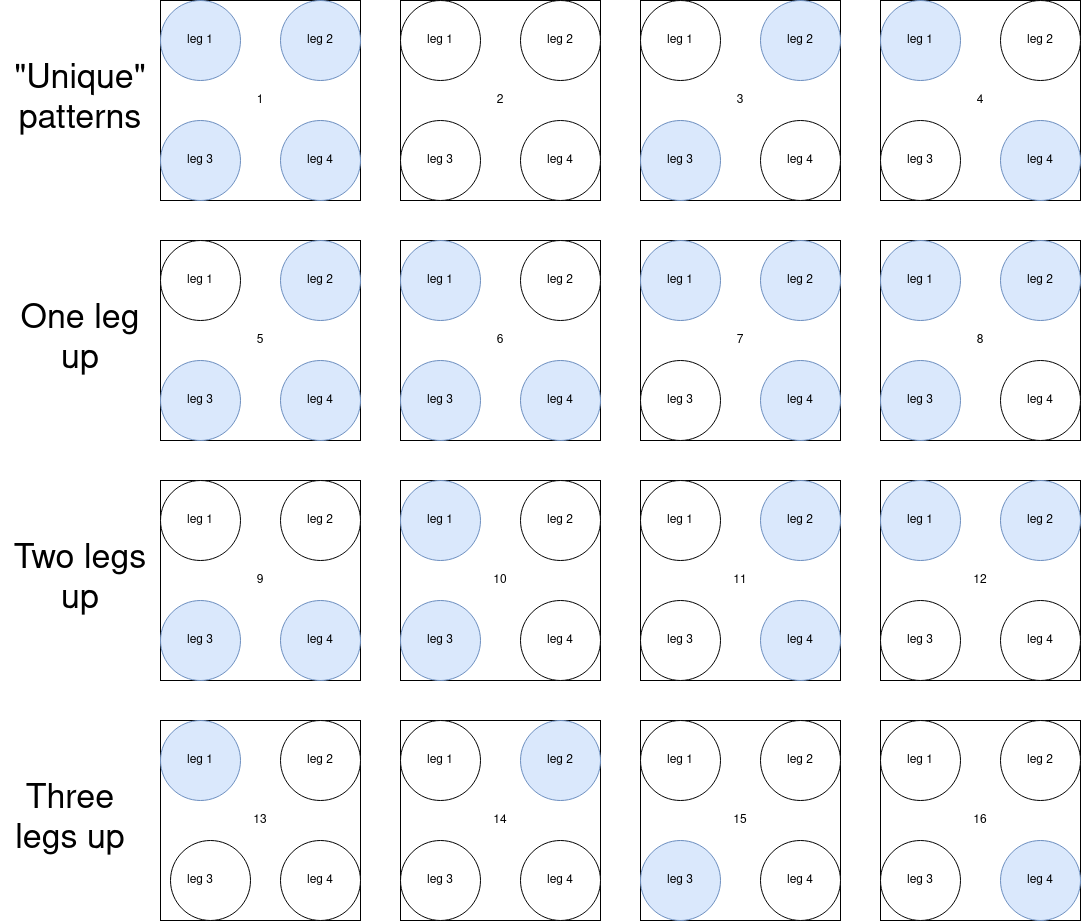
\includegraphics[width=0.5\textwidth]{img/gait.png}
    \caption{Blue means a leg is down and white is the leg is up}
    \label{gait}
\end{figure}

The gaits of a four legged robot is depicted in figure \ref{gait-walk}.
\begin{figure}[ht]
    \centering
    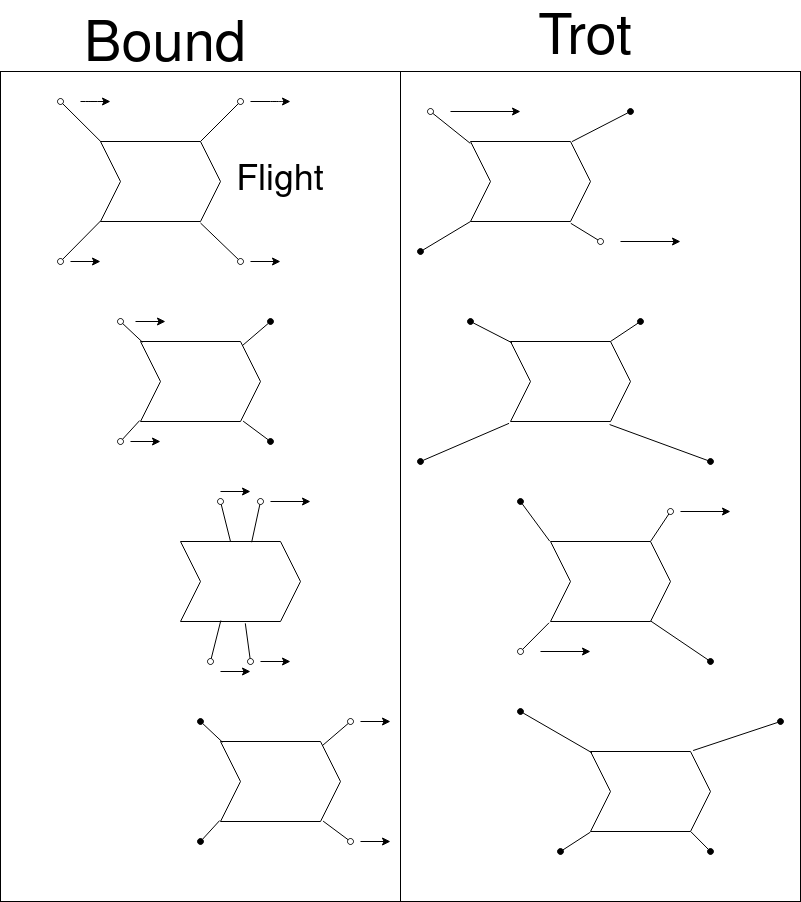
\includegraphics[width=0.4\textwidth]{img/gait-walk.png}
    \caption{The gaits of a 4 legged robot}
    \label{gait-walk}
\end{figure}
\newpage
%==============================================================================
\section*{Question 5}
% \textbf{\textit{
%     \tab Formulate the Monkey and Banana Problem in STRIPS:A monkey is at
%     location A in a lab. There is a box in location C. The monkey wants the
%     bananas that are hanging from the ceiling in location B, but it needs to
%     move the box and climb onto it in order to reach them 
% }} \\ \\
Note that the ways to represent STRIPS varies from source to source, and the
course content talks about the domain model. Considering the variance in the
representations of STRIPS, it was decided that doing the way that the course
content represents a domain model would be the best way. In the end, these
precise details about how the notation is done should not be a major concern as
long as it can be understood.
\subsection*{Predicates}
\begin{itemize}
    \item Location(?X) : X is a location
    \item BoxLocation(?X) : The box is at X
    \item Bananas(?X): X is bananas
    \item MonkeyLocation(?X) : Monkey is at X; can be a location or a box (given
    the monkey is on the box).
    \item Have(?X) : Monkey has X
    \item MonkeyOnBox(?X) : Monkey is on the box at location X
\end{itemize}
\subsection*{States}
\begin{itemize}
    \item \underline{Initial State} Location(A), Location(B), Location(C),
        Box(box), Bananas(bananas), BoxLocation(C), At(bananas, B),  
        MonkeyLocation(A) 
    \item \underline{Goal state} Have(bananas)
\end{itemize}
%//////////////////////////
\subsection*{World Operators}
\begin{itemize}
    \item MoveToLocation(?X, ?Y)
        \begin{itemize}
            \item Pre: Location(?X), Location(?Y), MonkeyLocation(?X)
            \item Effects+: MonkeyLocation(?Y)
            \item Effects-: MonkeyLocation(?X)
        \end{itemize}
    \item MoveBox(?X, ?Y)
        \begin{itemize}
            \item Pre: Location(?X), Location(?Y), MonkeyLocation(?X),
            BoxLocation(?X)
            \item Effects+: BoxLocation(?Y), MonkeyLocation(?Y)
            \item Effects+: BoxLocation(?X), MonkeyLocation(?X)
        \end{itemize}
    \item ClimbOnBox(?X)
        \begin{itemize}
            \item Pre: Location(?X), BoxLocation(?X), MonkeyLocation(?X),
            MonkeyOnBox(FALSE)
            \item Effects+: MonkeyOnBox(?X)
            \item Effects-: MonkeyLocation(?X) // this is to avoid situations
            where the monkey is on the box and tries to move. MonkeyLocation is
            technically set to null. We also don't need to program when the
            monkey climbs off the box as that's not necessary for its goal.
        \end{itemize}
    \item PickUpBanana(?X, ?Y)
        \begin{itemize}
            \item Pre: Banana(?X), Location(?Y),
                MonkeyLocation(?Y), MonkeyOnBox(?Y)
            \item Effects+: Have(?X)
            \item Effects-: 
        \end{itemize}
\end{itemize}
%==============================================================================
\section*{Question 6}
% \textbf{\textit{
%     \tab Evaluate  the  subsumption  architecture  in  terms  of:  support  for modularity, niche targetability, 
%     ease of portability to other domains, robustness
% }} \\ \\
% Modularity: Does it show good software engineering principles?
There are two perspectives on whether subsumption has good modularity.
Firstly, its granted hea  subsumption is a form of the reactive 
paradigm and its main architecture revolves around modules, 
it can be considered as highly modular. This is especially visible as 
modules are layered and reflects parts of object oriented programming as 
they have the ability to override, 
subsume and contain one another (when they're layered). 
Only thing that's arguably missing is inheritance, but 
that can probably be simulated by layering as well. \\
\tab The counter argument to this is that its very rarely
taken advantage of in practice when subsumption is used \cite{FangTang}. 
Overall, one would say there's more argument that its modularity is high as
it's capable of many OOP properties - even if it's rarely used.
\\
% Niche Targetability: How well does it work for the intended application? Lecture 5 1:20:18 he mentions this
\tab 
The niche targetability is high as we can design the system in a very specific way depending on the situation.
For instance, it can compile down onto a programmable-array logic circuit \cite{FangTang}.
\\
% Ease of portability to other domains: How well would it work for other applications or other robots? 1:21:55 lecture 5
\tab For portability, due to the fact that the system operates in layers 
if we tried to adjust an existing robot to a different application
chances are that it would take too much effort to do. As in, if 
there's a fundamental behaviour in layer 0, or even
the second last layer that we want to change it could be a lot 
of effort. On top of this, adapting to picking
different actions based on stimulus is challenging
For this reason its portability is quite low, which 
is different from a reactive paradigm. \cite{IntroToAI} \\
% Robustness: Where is the system vulnerable, and how does it try to reduce that vulnerability
\tab Overall its robustness to failure is arguable. 
Sensors failing is usually detected, and can be countered by having 
more than than the minimum number of sensors. 
Furthermore, the lower layers will continue to operate when higher ones
are added, however, the problem arises at high layers. 
These can only inhibit and suppress lower layers as they actively
interfere with them, and therefore they can cause undetected 
errors in the robot. Due to this its robustness is typically
evaluated as low because there is no inbuilt method to identify 
these failures. \cite{IntroToAI} \cite{reactiveParadigms}
\\
\tab In summary, it's modularity is good since it has many OOP functions and the niche targetability is high as it can be programmed
on very low level systems. 
It's main weakness out of the four is its ease of portability to different uses, and its robustness to failure
is generally considered low.

%==============================================================================
\newpage
\section*{Question 7}
% \textbf{\textit{
%     \tab Describe the Hybrid paradigm in terms of: (a) sensing, acting, and planning, and (b) sensing organization.
% }} \\ \\

Basically the planning is done on its own, and the sensing and acting are done together. That's to say that information,
sensed or cognitive, is put through the plan paradigm and that gives us directives. These directives allow our sense-act
section to decide what to do when it senses information. Its 'hybrid-ness' is visible through this, as it introduces
planning from other architectures into a reactive architecture's sensing and acting.
This assists with the downside of the subsumption model having difficulty adapting different actions 
to senses that are similar. The specific way P, SA acts is visible in figure \ref{HybridPSA}.
\begin{figure}[ht]
    \centering
    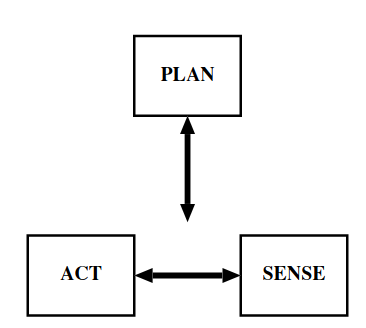
\includegraphics[scale=0.5]{img/PSA-Hybrid.png}
    \caption{The plan, sense act model for hybrid architecture}
    \label{HybridPSA}
\end{figure}

\tab The sensing organisation also merges the hierarchical and reactive styles as both planning and
acting requires the sensory
information. In the model this causes it to be more complex than the hierarchical one, our global world model can have its
own sensor and the behaviours can selectively listen to sensors while being able to create virtual sensors.
An example is visible in figure \ref{sOrg}.
\begin{figure}[ht]
    \centering
    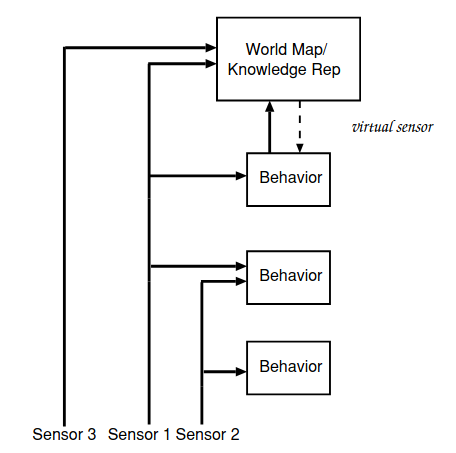
\includegraphics[scale=0.5]{img/sensing-organisation.png}
    \caption{Sensing organisation of hybrid paradigm. Taken from \cite{IntroToAI}}
    \label{sOrg}
\end{figure}
%==============================================================================
\newpage
\section*{Question 8}
% \textbf{\textit{
%     \tab Look up technical reports on Shakey. Compare Shakey with the Hybrid
% architectures.  Now  consider  the  possible  impact  of the  radical  increases  in
%  processing power since the 1960’s. Do you agree or disagree with the statement that
% Shakey would be as capable as any Hybrid if it were built today? Justify your answer.
% }} \\ \\
Shakey's initial model, made in the 1960's was designed using a hierarchical
paradigm and the second model slightly changed this \cite{shakeyHistory}. As
such, this question will be split into two sections due to the comparison being
different between both of these.
\subsection*{First Model - 1966}
The overwhelming issue with the first verson of shakey is the fact that
it effectively went blind when it was not in the sensing stage of its
plan-sensing-acting paradigm, which would happen to be majority of the time
\cite{IntroToAI}. This is due to both the hardware on board (SDS 940 computer
\cite{shakeyHistory}) and that the STRIPS paradigm is slow. For reference, a SDS
940 computer has a whopping maximum main of 64 kilowords and is old enough that
its processing speed was measured by microseconds to add numbers, not hertz.  \\

\tab To try to equate this to modern hardware, it takes 77 microseconds on the
SDS 940 to do a 24 bit floating operation. In other words it has (1/0.000077 =
12987 FLOPS(24 bit)(floating pointer operations per second)) \cite{SDS940}. 
On the other hand, an AMD Ryzen Threadripper 3990X has a whopping 13,209GFLOPS,
or 13209000000000 FLOPS (32bit) \cite{threadripper}. This massive difference
will allow a modern Shakey to spend next to no time in the planning stage.
\\
\tab However, in terms of the planning algorithmic speed, the hybrid
paradigm has O(n) algorithms \cite{IntroToAI}  
whereas STRIPS planning varies depending on the situation, but will always be 
PSPACE-complete; that is, it will never exceed $O(n^k)$ in complexity. This is
because hybrid models only plan up to the next stage, whereas a hierarchical
model plans everything from beginning to end, runs a small section of it, then
replans - even if it was correct \cite{shakey}.
\\
\tab However, even if we manage to keep up with STRIPS's much higher demand for
processing, the integral problem with it still exists: its single threaded. A
hybrid can see a situation, plan it, and while its acting if it goes wrong 
it can replan to react to the situation. On the other hand, STRIPS would finish
acting out its plan then realise something went wrong. An example is that say
Shakey is running to the bathroom, but a person walks in front of it - a hybrid
would instantly be able to react, while Shakey would finish its plan (driving
into you for a long time) and then realise something is wrong afterwards. For
this reason, the STRIPS model would have to be changed to compete with hybrid
robots. 
\subsection*{Second Model - 1971}
In the second model, Shakey was upgraded to a PDP-10 and due to this processing
improvement they changed the model into a layer hierarchical architecture. The
distinguishing feature of this is its capability to actually see while acting,
but the fact that its a five layered hierarchical system means it came with five
times the processing demand \cite{shakey}. In terms of big-O notation, this
isn't actually a visible change as the number of layers is just multiplied by
some constant ($O(cn^k) \rightarrow O(n^k)$. Good thing this is comparing it to
modern hardware which is billions of times faster. \\  
\tab Depending on the task, the revised Shakey would be equally as functional as a
hybrid robot. That's to say on an especially simple task it would be able to
complete it like a hybrid, but if a hybrid model even uses one percent of the
processor, the layered hierarchical model likely will not be able to handle
that. If we define capability by the bleeding edge functionalities of robots,
and the majority of those would use the entire processor if it can, then it
is not as capable as a hybrid model. \\ \\
\tab To sum it up, the first version fails to be as capable as a hybrid due to
its vision and time complexity while the revised version would not be as capable
because of the time complexity difference between linear and PSPACE-complete's
worst case.
\newpage

\bibliographystyle{apalike}
\bibliography{biblio}


\end{document}
